\documentclass[preprint]{article}

\usepackage{mathtools}
\usepackage{mathpartir}
\usepackage{fullpage}
\usepackage{ifpdf}
\usepackage{graphicx}
\usepackage[usenames,dvipsnames]{color}
\usepackage{subcaption}
\usepackage{stmaryrd}
\usepackage[numbers]{natbib}
\usepackage{amsthm}
\usepackage{listings}          % format code

\ifpdf
  \usepackage{hyperref}
  \usepackage{graphicx}
\else
  \usepackage[dvips]{graphicx}
  \usepackage[dvips]{hyperref}
\fi

\newcounter{copyrightbox}

% Math mode
%-----------
\newenvironment{nop}{}{}
\newenvironment{smathpar}{
\begin{nop}\small\begin{mathpar}}{
\end{mathpar}\end{nop}\ignorespacesafterend}

% Theorem
%--------
\newtheorem{theorem}{Theorem}

% Listings
%----------
\lstloadlanguages{haskell}
\newcommand{\lsthaskell}{\lstset{
      language=haskell,
      basicstyle=\ttfamily\ninett\footnotesize,
      flexiblecolumns=false,
			tabsize=2,
      %basewidth={0.5em,0.45em},
      %aboveskip={3pt},
      %belowskip={3pt},
      keywordstyle=\color{blue}\bfseries,
      commentstyle=\color{darkgreen}\itshape,
      morekeywords={foldl,fold},
			classoffset=1,
			upquote=true,
			keywordstyle=\color{Fuchsia}\bfseries,
			classoffset=0,
			mathescape=true,
      literate={+}{{$+$}}1 {/}{{$/$}}1 {*}{{$*$}}1 % {=}{{$=$}}1
               {>}{{$>$}}1 {<}{{$<$}}1
							 {dollar}{{\$}}1
               {\\\\}{{\char`\\\char`\\}}1
               {->}{{$\rightarrow$}}2 {>=}{{$\geq$}}2 {<-}{{$\leftarrow$}}2
               {<=}{{$\leq$}}2 {=>}{{$\Rightarrow$}}2
               {\ .}{{$\circ$}}2 {\ .\ }{{$\circ$}}2
               {>>}{{>>}}2 {>>=}{{>>=}}2 {=<<}{{=<<}}2
               {|}{{$\mid$}}1
							 {(-}{{$\in$}}1
						   {psi1}{{$\psi_1$}}1 {psi2}{{$\psi_2$}}1
							 {cup}{{$\cup$}}1
							 {cap}{{$\cap$}}1
							 {forall}{{$\forall$}}1
							 {vee}{{$\vee$}}1
							 {wedge}{{$\wedge$}}1
               {`member`}{{$\in$}}1
               {s.empty}{{\{\}}}1
               {leftbrace}{\{}1
               {rightbrace}{\}}1
               {profile0sing}{{ \{{\tt profile0}\}}}1
               {\$singleton\$startv}{{ \hspace{2.4em} \{{\tt startv}\}}}1
               {\$singleton\$n}{{  \{{\tt n}\}}}1
               {dotdotdot}{{$\ldots$}}3
    }}
\lstnewenvironment{codehaskell}
    { % \centering
			\lsthaskell
      \lstset{}%
      \csname lst@setfirstlabel\endcsname}
    { %\centering
      \csname lst@savefirstlabel\endcsname}

\newcommand{\lstml}{
\lstset{ %
language=ML, % choose the language of the code
basicstyle=\small\ttfamily,       % the size of the fonts that are used for the code
keywordstyle=\color{Bittersweet},
% numbers=left,                   % where to put the line-numbers
numberstyle=\tiny,      % the size of the fonts that are used for the line-numbers
stepnumber=1,                   % the step between two line-numbers. If it is 1 each line will be numbered
numbersep=5pt,                  % how far the line-numbers are from the code
showspaces=false,               % show spaces adding particular underscores
showstringspaces=false,         % underline spaces within strings
showtabs=false,                 % show tabs within strings adding particular underscores
% frame=single,                   % adds a frame around the code
tabsize=2,                      % sets default tabsize to 2 spaces
captionpos=b,                   % sets the caption-position to bottom
breaklines=true,                % sets automatic line breaking
breakatwhitespace=false,        % sets if automatic breaks should only happen at whitespace
commentstyle=\itshape\color{MidnightBlue},
%escapeinside={\%*}{*)},         % if you want to add a comment within your code
morekeywords={relation, not, : , /\\}
}}
\lstnewenvironment{codeml}
    { % \centering
			\lstml
      \lstset{}%
      \csname lst@setfirstlabel\endcsname}
    { %\centering
      \csname lst@savefirstlabel\endcsname}
% Formatting
%---------
\newcommand{\C}[1]{\code{#1}}
\newcommand{\tuplee}[1]{\langle #1 \rangle}
\newcommand*{\rom}[1]{\expandafter\romannumeral #1}

% Formatting commands
% -------------------
\newcommand{\code}[1]{\,{\tt #1}\,}
\newcommand{\spc}[0]{\quad}
\newcommand{\ALT}{~\mid~}
\newcommand{\rel}[1]{{R}_{\mathit{#1}}}
\newcommand{\conj}{\wedge}
\newcommand{\disj}{~\vee~}
\newcommand{\rulelabel}[1]{\textrm{\sc {#1}}}
\newcommand{\ilrulelabel}[1]{{\sc #1}}
\newcommand{\RULE}[2]{\frac{\begin{array}{c}#1\end{array}}
                           {\begin{array}{c}#2\end{array}}}
\newcommand{\denot}[1]{\llbracket #1 \rrbracket}
\date{}
\begin{document}

\title{DaLi - Concurrency Model}
%\subtitle{Research Summary}

% \author{Gowtham Kaki \\ \small{Purdue University} \hspace*{0.1in}
%   \small{{\tt gkaki@purdue.edu}} }

\maketitle

\section{Introduction}

In this document, I describe the concurrency model of dali, and ways
to realize it on single and distributed machines.

\section{The Branch Concurrency Model}

\begin{figure}[ht]

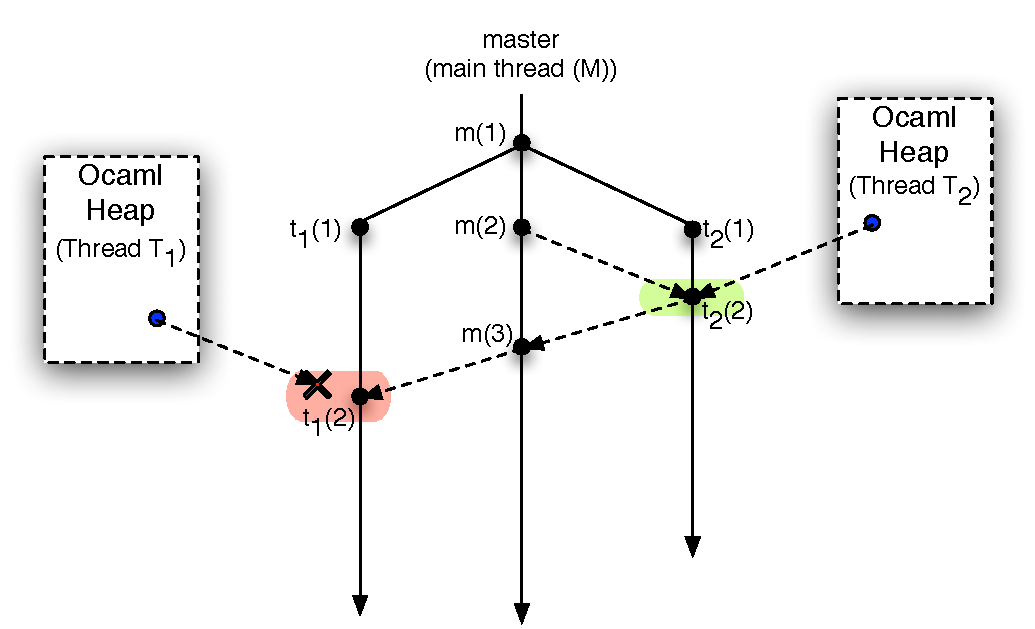
\includegraphics[scale=0.75]{Figures/sync-1}

\caption{The branch concurrency model with a simple two-level
hierarchy}
\label{fig:sync-1}
\end{figure}

A DaLi program consists of multiple concurrent threads operating on a
persistent shared state. The OCaml type of the shared state
distinguishes it from the thread-local state. Unlike imperative
programs, where the there exists a single copy of the shared state
that is \emph{updated} by concurrent threads, DaLi programs manage
shared state in a fashion similar to the version control software,
i.e., by \emph{forking} off new (concurrent) versions and
\emph{merging} them back. We refer to a totally-ordered sequence of
versions as a \emph{branch}. The program starts execution in its main
thread with an initial version of the shared state, which is the first
version of the \emph{master} branch. Certain operations performed by
the program (described later) result in the creation of later versions
on the master branch. Forking off new threads by the program results
in forking off new versions of the state along the new branches; each
thread is associated a new branch. In Fig.~\ref{fig:sync-1} for
example, main thread ($M$) operating on the master branch ($m$)
creates two new threads - $T_1$ and $T_2$, which fork off two new
branches - $t_1$ and $t_2$, respectively. The first versions on both
the branches, i.e., $t_1(1)$ and $t_2(1)$, denote the same state (same
as the forked version $m(1)$ on the master), yet the versions themselves
are deemed distinct and concurrent. Formally, $t_1(1) \neq t_2(1) \neq
m(1)$, but $\denot{t_1(1)} = \denot{t_2(1)} = \denot{m(1)}$.
% Note that the thread fork operation is blocking; the caller thread
% blocks until all the child threads finish execution and return. 

The concurrency model allows threads to periodically synchronize their
branches with the master branch via the \C{sync\_next\_version}
operation. The operation is so named because it synchronizes the
immediate next version on the caller thread's branch with a version on
the master that is later than (or same as) the last master version
known to the branch. Concurrent threads that only serve read requests
are expected to periodically sync with the master to contain the
staleness of the data served. However, threads may also wish to
write new data and make it available globally. For this purpose,
\C{sync\_next\_version} allows the caller to (optionally) pass an
argument proposing the next version of the state. If there haven't
been any later versions on the master since the last known version,
the proposal is accepted and published as the next version on the
branch, and also the master. If there have been later master versions,
then latest such version is merged with the proposed version and
published. For this reason, applications are expected to implement a
merge function for the type of the state. In Fig.~\ref{fig:sync-1},
thread $T_2$ proposes a new version (the blue dot), which is merged
with the version $m(2)$ of the master (merge highlighted in the green
background), and the result is published as the version $t_2(2)$ on
the $t_2$ branch and $m(3)$ on the master branch. It may sometimes
transpire that the version proposed by the thread may be in conflict
with the latest version on the master, in which case the merge
function is allowed to return an error value and fail. This scenario
is captured in Fig.~\ref{fig:sync-1} in the red background. The
failure of merge results in the thread's proposal not being accepted,
and master's version being published as the next version on the
branch. In Fig.~\ref{fig:sync-1}, the failure of merge in $T_1$
results in master's $m(3)$ getting published as $t_1(2)$ on $t_1$.
Note that this version denotes the same state as present on the $t_2$
branch, which incorporates $T_2$'s proposal, thus demonstrating the
information flow among the branches.

The threads can access the lastest version on their branches via the
\C{get\_latest\_version} operation. If the last merge operation is a
success, then this operation returns the merged version, allowing the
thread to continue its computation. If the last merge operation
failed, then it allows the thread to read the latest version of the 
master and revise its proposal for the next \C{sync} operation. 

The behavior of \C{sync\_next\_version} and \C{get\_latest\_version}
is more-or-less same in the main thread. While \C{sync} without a
propoisal is effectively a \C{nop} in the main thread, a \C{sync} with
a proposal tries to merge the proposal with the lastest master
version, which happens to be the local version for the main thread. As
with other threads, \C{sync} fails if the proposed version is
incompatible with the later version. There is however a slight
difference in behavior of the \C{get\_latest\_version} in the main
thread; unlike in other threads, successive calls to
\C{get\_latest\_version} in the main thread may return different
results even if they are not interleaved by a \C{sync} operation. This
happens if one of the child threads syncs its branch with the master
inbetween the two calls.

\subsection{Generalizing to branch hierarchies of any depth}

\begin{figure}[t]
\centering
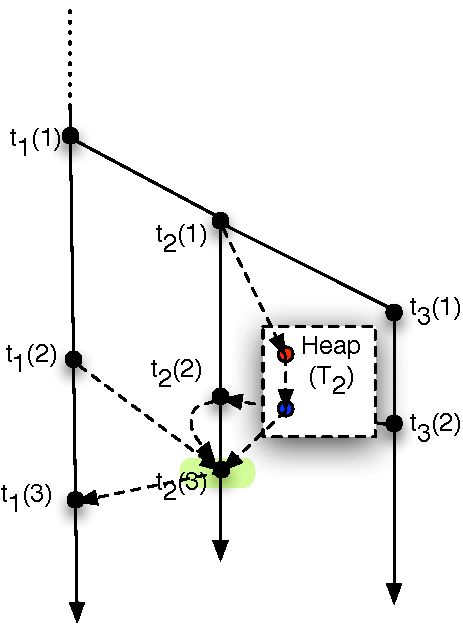
\includegraphics[scale=0.75]{Figures/sync-2}

\caption{The branch concurrency model generalized to hierarchies of
any depth}
\label{fig:sync-2}
\end{figure}

Observe that the branch concurrency model desribed above confines
branching to a 2-level hierarchy with the master branch at the top and
forked branches at the bottom. The model does not define the behavior
of the version/thread fork operation originating from one of the child
threads. We now generalize the model for branch hierarchies of any
depth, while also eliminating the slight asymmetry between the main
thread and the child threads described above. We achieve this
generalization by redefining the \C{sync\_next\_version} operation as
a two-step process that first merges the proposed version with the
latest version on the current branch, and then merges the result with
the latest version on the parent branch (note: not necessarily the
master branch). The additional first step is now necessary because the
latest version on the current branch may not be same as the one that
was last read through the \C{get\_latest\_version}; a new version may
have since been committed by one of the child threads of the current
thread. The first step merges the proposed version with this version.
The second stepe merges the result of the first step with the lastest
version on the master, and publishes the merge result on both the
branches.

In Fig.~\ref{fig:sync-2}, thread $T_1$ forks a child $T_2$, which
forks $T_3$. The initial versions on the corresponding branches are
$t_1(1)$, $t_2(1)$, and $t_3(1)$, respectively. Thread $T_2$ starts a
local computation on its initial version copied into its heap (the red
dot). At some point, $T_3$ publishes a later version ($t_2(2)$) to its
parent. A little while later, $T_2$ concludes its local computation
and proposes a candidate for the new version on $t_2$ (the blue dot;
the dotted line connecting the red and blue dots denotes data
dependency). This candidate is merged with the latest local version
($t_2(2)$), and also the latest parent version ($t_1(2)$), and the
merge result\footnote{Convergence requires merge to be commutative, so
the order of merging doesn't matter.} is published as $t_2(3)$ on the
local branch and $t_1(3)$ on the parent branch. Subsequence
\C{get\_latest\_version} returns these versions on both the branches.

Observe that the behavior of \C{sync\_next\_version} and
\C{get\_latest\_version} is now uniform across all the threads. The
first and second steps (resp.) of \C{sync\_next\_version} are
effectively nop for the root and leaves of the thread hierarchy,
because the master branch doesn't have a parent and the bottom-most
branch doesn't have a child.
the main thread doesn't have a parent,

\subsection{Blocking sync only when necessary}

One problem with the previous model is that the call to
\C{sync\_later\_version} always blocks until the merge operation
succeeds and the result is published on both the branches. This is
unnecessary if the merge operation is always guaranteed to succeed (for
e.g., in the case of a mergeable queue). A non-blocking \C{sync} is
more appropriate for such cases. Selective non-blocking behavior for
can be accommodated in the semantics of \C{sync} as following: Along
with the proposal for the later version, \C{sync} also accepts the
current continuation of the caller. If there is a possiblity that any
of the two merge operations might fail, then \C{sync} waits until it
obtains the result of merges before calling the continuation with an
appropriate status.  Otherwise, it calls the current continuation
immediately, reporting success status. Some subsequent (but not
necessarily immediate) call to \C{get\_latest\_version} is guaranteed
to return the merged version\footnote{This guarantee is conditional on
the EC guarantee of the underlying machine and the commutativity
property of the merge function.}.

But how does the \C{sync} know if the merge might return conflict? By
observing the diff (\C{git diff}) of the proposed and the latest local
versions w.r.t to the last known version of the parent. For example,
let us consider an application whose shared state contains three data
items - \C{x}, \C{y}, and \C{z}, which are indepedently mergeable. Suppose
that the type of the merge function for \C{z} indicates a possibility of
conflict (\C{type 'a result = Ok of 'a | Conflict}), whereas the merge
functions for \C{x} and \C{y} do not admit that possibility. Let the last
know parent version be \C{\{x=a; y=b; z=c\}}, the latest local version
be \C{\{x=a'; y=b'; z=c\}}, and the proposed version be \C{\{x=a''; y=b;
z=c\}}. It is clear that the merge function on \C{z} will not be called
while merging the versions, hence there is not possibility that the
merge fails. Consequencely, \C{sync} can be non-blocking in this case.
On the other hand, if \C{z} is assigned \C{c'} in the proposed version,
then the merge on \C{z} will be called, which might fail. Therefore,
\C{sync} needs to block.

The banality of selective blocking optimization belies its true
importance, for the selectively blocking \C{sync} is what lets DaLi
implement a highly available replicated data store with on-demand
strong consistency, without requiring programmers to explicitly reason
about the consistency.  

\section{Operational Semantics}

\begin{figure*}[!t]
\raggedright
%
\textbf{Syntax}\\
%
\begin{smathpar}
\renewcommand{\arraystretch}{1.2}
\begin{array}{lclcl}
\multicolumn{5}{c} {
  t \in \mathtt{Thread\; Ids} \qquad
  x,y \in \mathtt{Variables} \qquad
  c \in \mathtt{\{()\}} \cup \mathbb{N} \qquad
}\\
v & \in & \mathtt{Values} & \coloneqq & c \ALT \lambda x.\,s\\
s & \in & \mathtt{Expressions} & \coloneqq & v \ALT s\;s \ALT \run{s}{s}
   \ALT \fork{s} \ALT \pull \ALT \push{s}\\
p & \in & \mathtt{Programs} & \coloneqq & s_t \ALT p\,||\,p \\
f & \in & \mathtt{Tags} & \coloneqq & \C{INIT} \ALT \C{FORK} \;b 
  \ALT \C{PUSH} \ALT \C{MERGE} \;b\\
b & \in & \mathtt{Branches} & \coloneqq & [(v,f)] \ALT (v,f)::b \\
\end{array}
\end{smathpar}
%
\bigskip
%% If we are feeling adventurous, we can try defining e and s 
%% mutually recursively, such that their evaluation relations 
%% are also mutually recursive (multiple reduction steps of one 
%% relation is a single step of other). 

%
\textbf{Evaluation Contexts}\\
%
\begin{smathpar}
\renewcommand{\arraystretch}{1.2}
\begin{array}{lclcl}
H & \in & \mathtt{Branch\; Histories} & \coloneqq & t \mapsto b\\
E & \in & \mathtt{Eval.\; Contexts}(s) & \coloneqq & \bullet \ALT 
  \bullet\;s \ALT v\;\bullet \ALT \run{\bullet}{s}\\
P & \in & \mathtt{Eval.\; Contexts}(p) & \coloneqq & E_t \ALT 
  \bullet\,||\,p \ALT p\,||\,\bullet \\
\end{array}
\end{smathpar}
%
\bigskip

%
\textbf{Reduction Relation} \quad \fbox {$p;\;H \stepsto p';\;H'$} \\
%
%
\begin{smathpar}
\begin{array}{lcll}
(\run{v}{s})_t;\cdot & \stepsto & 
  s_t; \cdot[t_{\top} \mapsto [(v,\C{INIT})]]
            [t\mapsto [(v,\C{FORK}\; [(v,\C{INIT})])]] 
            & [\rulelabel{E-Run}]\\
(\fork{s})_t;H(t\mapsto (v,\_)::b) & \stepsto & 
    ()_t\,||\, s_{t'}; H[t'\mapsto [(v, \C{FORK} H(t))]] 
    \spc \texttt{where}\; t'\not\in dom(H)
            & [\rulelabel{E-Fork}]\\
(\push{v})_t;H & \stepsto & ()_t;H[t \mapsto (v,\C{PUSH})::H(t)]
            & [\rulelabel{E-Push}]\\
% & & & v\,=\,\C{merge}\,v\,v_1\,v_2 ~\texttt{and}~ \\
((\lambda x.s)\;v)_t;H & \stepsto & ([v/x]\,s)_t;H
            & [\rulelabel{E-App}]\\
(\pull)_t;H(t \mapsto (v,\_)::m) & \stepsto & v_t;H
            & [\rulelabel{E-Pull}]\\
\end{array}
\end{smathpar}
%

% %
% \hspace*{\fill}[\rulelabel{E-Admin}]\hspace*{0.25in}
% \begin{smathpar}
% \begin{array}{c}
% \RULE
% {
%   s_t; H ~\stepsto^{*}~ v_t; H
% }
% {
%   E_t[s]; H ~\stepsto^{*}~ E_t[v]; H
% }
% \end{array}
% \end{smathpar}
% %

%
\hspace*{\fill}[\rulelabel{E-Pull-Wait}]
\begin{smathpar}
\begin{array}{c}
\RULE
{
  t\neq t' \spc
  \under{H}{v' \mbleto v} \spc
% \C{world}(H,t') \semsucceq \C{world}(H,t)\spc 
  v_m = \C{merge}(\C{lca}(H(t),H(t')), v, v') \spc
}
{
  (\pull)_t;H(t \mapsto (v,f)::m)(t' \mapsto (v',\_)::\_) ~\stepsto~
  (\pull)_t;H[t \mapsto (v_m,\C{MERGE}\; H(t'))::(v,f)::m]
}
\end{array}
\end{smathpar}
%

\caption{\name: Syntax and Operational Semantics}
\label{fig:opsem}
\end{figure*}


\begin{figure}[!h]
\begin{smathpar}
\begin{array}{lcll}
(\push{v_1}, v::b)_t;M[t\mapsto v_2::m] & \stepsto & 
    ((),v_1::v::b)_t;M[t \mapsto v'::v_2::m] & \texttt{where}~
    t\neq t'~\texttt{and}\\
  & & & v\,=\,\C{merge}\,v\,v_1\,v_2 ~\texttt{and}~ \\
\end{array}
\end{smathpar}

\begin{smathpar}
\begin{array}{c}
\RULE
{
  t\neq t' \spc
  v_1 \not\succeq v_2 \conj v_2 \not\succeq v_1 \spc
  v = \C{merge}(\C{lca}(M(t),M(t')), v_1, v_2)
}
{
  (s,b)_t;M[t\mapsto v_1::m_1][t'\mapsto v_2::m_2] ~\stepsto~
  (s,b)_t;M[t \mapsto v::v_1::m_1][t'\mapsto v_2::m_2]
}
\end{array}
\end{smathpar}
%

\caption{DaLi: Low-level Operational Semantics}
\label{fig:low-opsem}
\end{figure}



\section{Instantiations}

DaLi's concurrency model is general enough that it can be instantiated
in system-specific ways. 

\subsection{Single-node database}

ToDo.

\subsection{Replicated data store}

ToDo.



{
%\small
\bibliographystyle{plainnat} \small \bibliography{report}
}

\end{document}

